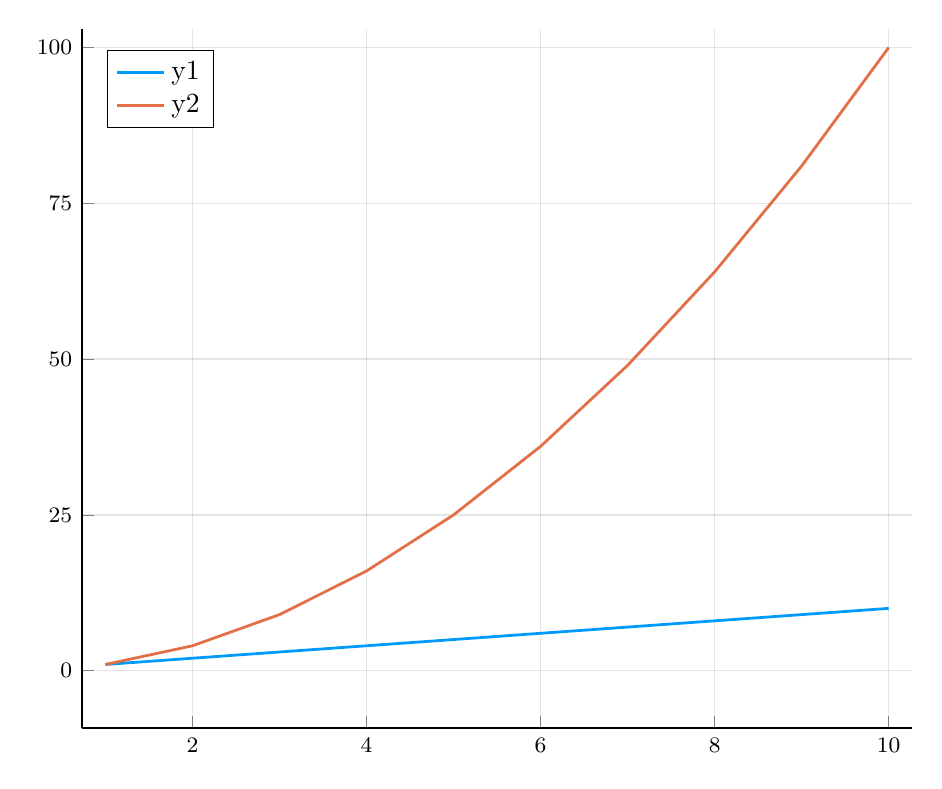
\begin{tikzpicture}[]
\begin{axis}[
    width = \columnwidth,
    ylabel = {},
    xmin = {0.73},
    xmax = {10.27},
    ymax = {102.97},
    xlabel = {},
    unbounded coords=jump,
    scaled x ticks = false,
    xlabel style = {font = {\fontsize{11 pt}{14.3 pt}\selectfont}, color = {rgb,1:red,0.00000000;green,0.00000000;blue,0.00000000}, draw opacity = 1.0, rotate = 0.0},
    xmajorgrids = true,
    xtick = {2.0,4.0,6.0,8.0,10.0},
    xticklabels = {$2$,$4$,$6$,$8$,$10$},
    xtick align = inside,
    xticklabel style = {
        font = {\fontsize{8 pt}{10.4 pt}\selectfont},
        color = {rgb,1:red,0.00000000;green,0.00000000;blue,0.00000000},
        draw opacity = 1.0,
        rotate = 0.0},
    x grid style = {
        color = {rgb,1:red,0.00000000;green,0.00000000;blue,0.00000000},
        draw opacity = 0.1,
        line width = 0.5,
        solid},
    axis x line* = left,
    x axis line style = {
        color = {rgb,1:red,0.00000000;green,0.00000000;blue,0.00000000},
        draw opacity = 1.0,
        line width = 1,
        solid},
    scaled y ticks = false,
    ylabel style = {
        font = {\fontsize{11 pt}{14.3 pt}\selectfont},
        color = {rgb,1:red,0.00000000;green,0.00000000;blue,0.00000000},
        draw opacity = 1.0,
        rotate = 0.0},
    ymajorgrids = true,
    ytick = {0.0,25.0,50.0,75.0,100.0},
    yticklabels = {$0$,$25$,$50$,$75$,$100$},
    ytick align = inside,
    yticklabel style = {font = {\fontsize{8 pt}{10.4 pt}\selectfont},
    color = {rgb,1:red,0.00000000;green,0.00000000;blue,0.00000000},
    draw opacity = 1.0, rotate = 0.0},
    y grid style = {
        color = {rgb,1:red,0.00000000;green,0.00000000;blue,0.00000000},
        draw opacity = 0.1,
        line width = 0.5,
        solid},
    axis y line* = left,
    y axis line style = {color = {rgb,1:red,0.00000000;green,0.00000000;blue,0.00000000},
        draw opacity = 1.0,
        line width = 1,
        solid},
    xshift = 0.0mm,
    yshift = 0.0mm,
    axis background/.style={fill={rgb,1:red,1.00000000;green,1.00000000;blue,1.00000000}},
    legend pos = {north west}
]

\addplot+ [
    color = {rgb,1:red,0.00000000;green,0.60560316;blue,0.97868012},
    draw opacity = 1.0,
    line width = 1,
    solid,
    mark = none,
    mark size = 2.0,
    mark options = {
            color = {rgb,1:red,0.00000000;green,0.00000000;blue,0.00000000}, draw opacity = 1.0,
            fill = {rgb,1:red,0.00000000;green,0.60560316;blue,0.97868012}, fill opacity = 1.0,
            line width = 1,
            rotate = 0,
            solid
        }] coordinates {
(1.0, 1.0)
(2.0, 2.0)
(3.0, 3.0)
(4.0, 4.0)
(5.0, 5.0)
(6.0, 6.0)
(7.0, 7.0)
(8.0, 8.0)
(9.0, 9.0)
(10.0, 10.0)
};
\addlegendentry{y1}
\addplot+ [
    color = {rgb,1:red,0.88887350;green,0.43564919;blue,0.27812294},
    draw opacity = 1.0,
    line width = 1,
    solid,mark = none,
    mark size = 2.0,
    mark options = {
            color = {rgb,1:red,0.00000000;green,0.00000000;blue,0.00000000}, draw opacity = 1.0,
            fill = {rgb,1:red,0.88887350;green,0.43564919;blue,0.27812294}, fill opacity = 1.0,
            line width = 1,
            rotate = 0,
            solid
        }]coordinates {
(1.0, 1.0)
(2.0, 4.0)
(3.0, 9.0)
(4.0, 16.0)
(5.0, 25.0)
(6.0, 36.0)
(7.0, 49.0)
(8.0, 64.0)
(9.0, 81.0)
(10.0, 100.0)
};
\addlegendentry{y2}
\end{axis}

\end{tikzpicture}
